\begin{center}
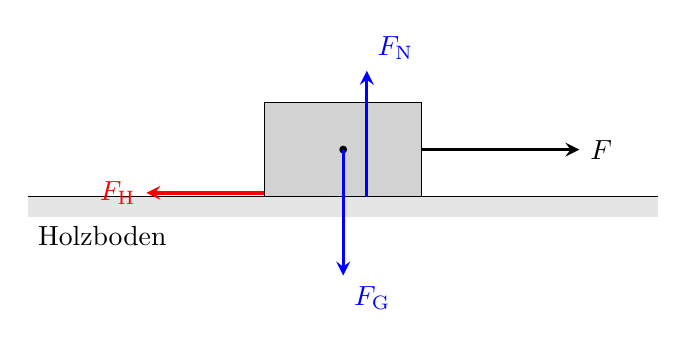
\begin{tikzpicture}[>=stealth]
 \fill[gray!20] (-4,0) rectangle (4,-0.25);
 \draw (-4,0) -- (4,0);
 \node[anchor=north west] at (-4,-0.25) {Holzboden};
 \draw[fill=gray!35] (-1,0) rectangle (1,1.2);
 \fill (0,0.6) circle (0.05);
 \draw[->, very thick] (1,0.6) -- ++(2.0,0) node[right] {$F$};
 \draw[->, very thick, red] (-1,0.05) -- ++(-1.5,0) node[left] {$F_\mathrm{H}$};
 \draw[->, very thick, blue] (0,0.6) -- ++(0,-1.6) node[anchor=north west] {$F_\mathrm{G}$};
 \draw[->, very thick, blue] (0.3,0) -- ++(0,1.6) node[anchor=south west] {$F_\mathrm{N}$};
\end{tikzpicture}
\end{center}

Solange der Schrank ruht, ist die Haftreibungskraft gleich gross wie die horizontale Kraft $F$. Sie kann aber höchstens $\mu_\mathrm{H}\,F_\mathrm{N}$ betragen. Für Holz auf Holz ist $\mu_\mathrm{H} = \muHO$ (FoTaBe S.~189), und auf dem horizontalen Boden ist $F_\mathrm{N} = m\,g$. Der Schrank beginnt zu rutschen, sobald
\begin{align}
 F &> \FZuF \\
   &= \muH\cdot\mSc\cdot\gE \\
   &= \FZu \approx \result{\FZuP{0}{2}}
\end{align}
Die Haftreibungszahl von Holz auf Holz streut stark (FoTaBe: $\pm\dmuO$), das Resultat ist deshalb nur ein Richtwert.
